\section{Exploratory Data Analysis}
\label{sec:formatting}

%------------------------------------------------------------------------
\subsection{Question Length Distribution Across Datasets}
The graph in Fig. 3 indicates that the majority of questions in both the training and validation sets of the VQA v2 dataset consist of 4 to 7 words, with the distributions almost overlapping, implying the validation set's representativeness of the training set. Conversely, questions in the DAQUAR dataset tend to be longer, primarily falling within the range of 6 to 11 words.

\begin{figure}[htbp]
  \centering
   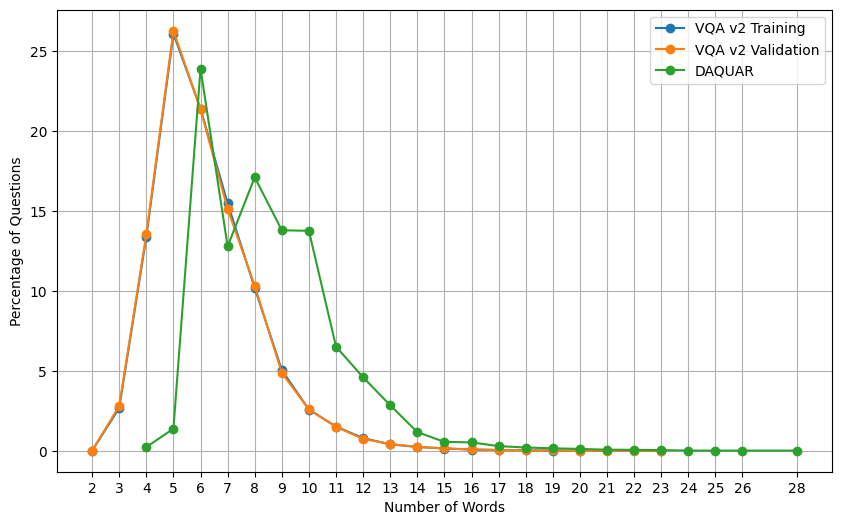
\includegraphics[width=\linewidth]{sec/Images/image3.png}
   \caption{}
   \label{fig:onecol}
\end{figure}

\subsection{Answer Length Distribution Across Datasets}
The graph in Fig. 4 reveals that the majority of answers in both the VQA v2 datasets (training and validation sets) and the DAQUAR dataset consist of 1 or 2 words. This could suggest that the questions are designed to elicit simple or direct information from the images, rather than requiring complex or elaborate explanations.

\begin{figure}[htbp]
  \centering
   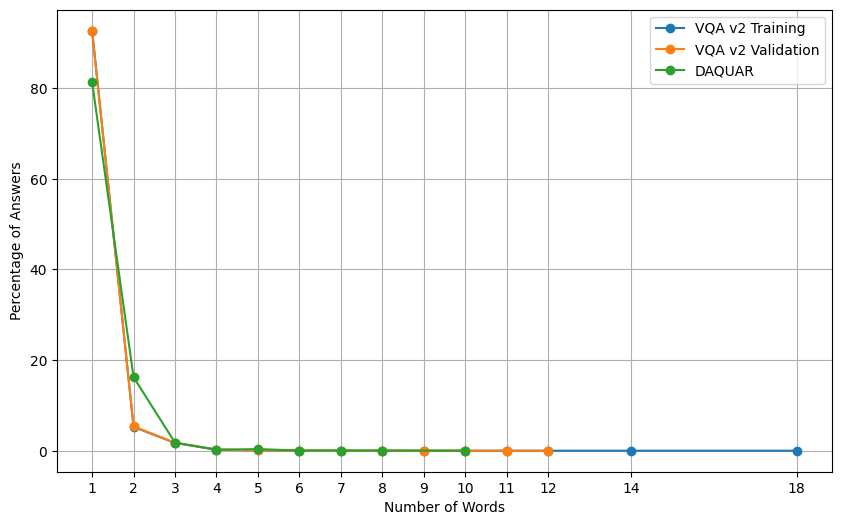
\includegraphics[width=\linewidth]{sec/Images/image4.png}
   \caption{}
   \label{fig:onecol}
\end{figure}

\subsection{Question Type Distribution Across Datasets}
The graph in Fig. 5 provides insights into the design of questions within the datasets. In the VQA v2 datasets (both training and validation sets), questions starting with “how many,” “is the,” and “what” are predominant. Conversely, in the DAQUAR dataset, questions frequently begin with “what is on the,” “what is the,” and “what is.” This suggests a focus on different types of queries in each dataset, with VQA v2 emphasising queries about quantity, state, and general attributes, while DAQUAR leans towards inquiries about object identification and description.



\begin{figure}[htbp]
  \centering
   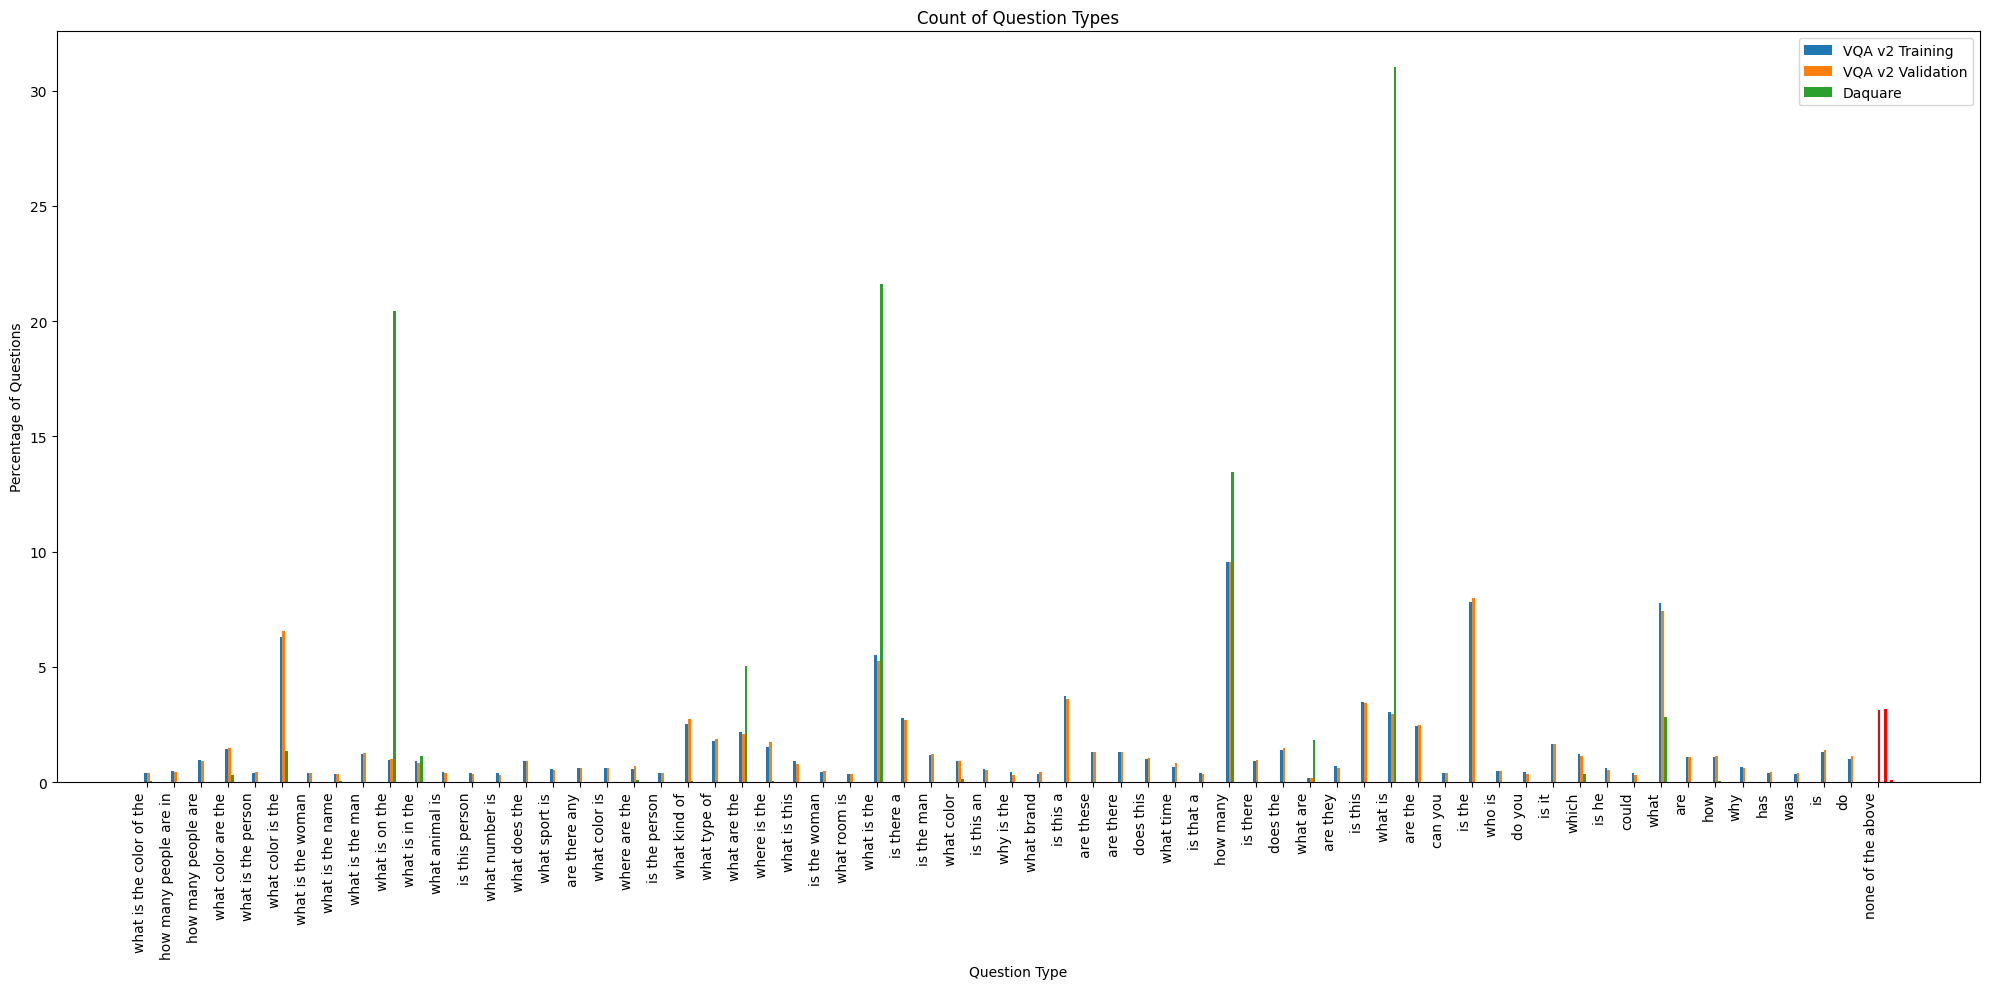
\includegraphics[width=\linewidth]{sec/Images/image5.png}
   \caption{}
   \label{fig:onecol}
\end{figure}

%-------------------------------------------------------------------------
